\documentclass[tikz,border=8pt]{standalone}
\usetikzlibrary{arrows.meta,calc,decorations.pathmorphing}

\begin{document}
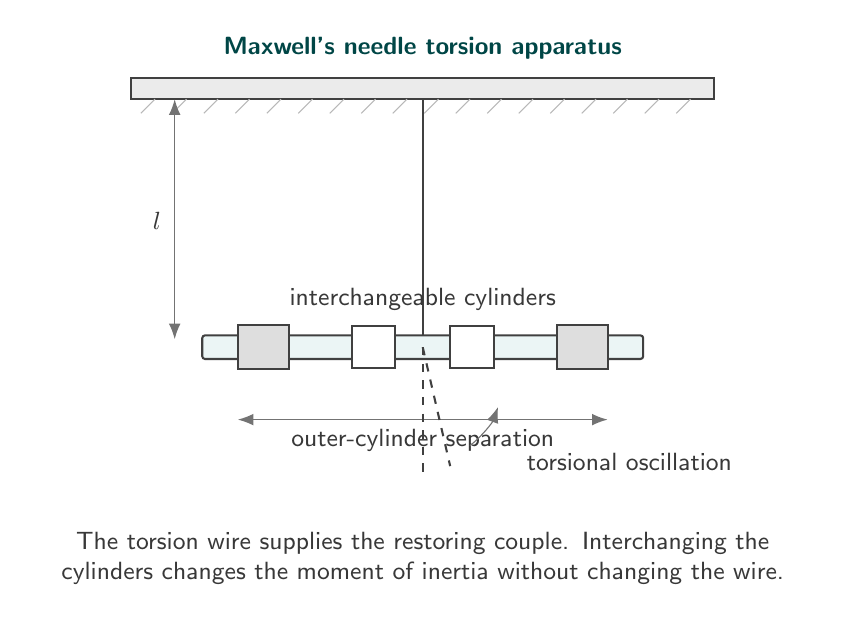
\begin{tikzpicture}[
  line/.style={draw=black!75,line width=0.75pt},
  label/.style={font=\sffamily\small,text=black!78},
  title/.style={font=\sffamily\bfseries\small,text=teal!55!black},
  dim/.style={{Latex[length=2mm]}-{Latex[length=2mm]},draw=black!55,line width=0.55pt},
]

\node[title] at (0,4.2) {Maxwell's needle torsion apparatus};
\draw[line,fill=black!8] (-3.7,3.55) rectangle (3.7,3.82);
\foreach \x in {-3.4,-3.0,...,3.4}
  \draw[black!28] (\x,3.55) -- ++(-0.18,-0.18);

\draw[line] (0,3.55) -- (0,0.5);
\draw[line,fill=teal!8,rounded corners=1pt] (-2.8,0.25) rectangle (2.8,0.55);
\draw[line,fill=black!13] (-2.35,0.12) rectangle (-1.7,0.68);
\draw[line,fill=black!13] (1.7,0.12) rectangle (2.35,0.68);
\draw[line,fill=white] (-0.9,0.13) rectangle (-0.35,0.67);
\draw[line,fill=white] (0.35,0.13) rectangle (0.9,0.67);
\node[label,above] at (0,0.74) {interchangeable cylinders};

\draw[dim] (-3.15,3.55) -- (-3.15,0.5);
\node[label,left] at (-3.2,2.0) {$l$};
\draw[dim] (-2.35,-0.52) -- (2.35,-0.52);
\node[label,below] at (0,-0.52) {outer-cylinder separation};

\draw[line,dashed] (0,0.4) -- (0,-1.25);
\draw[line,dashed,rotate around={13:(0,0.4)}] (0,0.4) -- (0,-1.15);
\draw[-{Latex[length=2mm]},draw=black!55] (0.6,-0.85) arc[start angle=-52,end angle=-20,radius=1.1];
\node[label,right] at (1.2,-1.05) {torsional oscillation};

\node[label,align=center,text width=9.8cm] at (0,-2.28)
  {The torsion wire supplies the restoring couple. Interchanging the cylinders changes the moment of inertia without changing the wire.};

\end{tikzpicture}
\end{document}
